\documentclass[10pt]{article}
\usepackage[english]{babel}
\usepackage{amsmath}
\usepackage{graphicx}
\usepackage[colorinlistoftodos]{todonotes}
\pagestyle{headings}
\usepackage{indentfirst}
\usepackage[utf8]{inputenc}
\usepackage{xeCJK}
\usepackage{float}
\usepackage {subcaption}

%% Code blocl setting
\usepackage{listings}
\renewcommand{\lstlistingname}{Code}% Listing -> Algorithm
\usepackage{color}

\definecolor{dkgreen}{rgb}{0,0.6,0}
\definecolor{gray}{rgb}{0.5,0.5,0.5}
\definecolor{mauve}{rgb}{0.58,0,0.82}

\lstset{frame=tb,
  language=Python,
  aboveskip=3mm,
  belowskip=3mm,
  showstringspaces=false,
  columns=flexible,
  basicstyle={\small\ttfamily},
  numbers=none,
  numberstyle=\tiny\color{gray},
  keywordstyle=\color{blue},
  commentstyle=\color{dkgreen},
  stringstyle=\color{mauve},
  breaklines=true,
  breakatwhitespace=true,
  tabsize=3
}

\begin{document}

\begin{titlepage}

\newcommand{\HRule}{\rule{\linewidth}{0.5mm}} % Defines a new command for the horizontal lines, change thickness here

\center % Center everything on the page

%----------------------------------------------------------------------------------------
%	HEADING SECTIONS
%----------------------------------------------------------------------------------------

\textsc{\LARGE Shanghai Jiaotong University}\\[1.5cm] % Name of your university/college
\textsc{\Large Visual Scene Real-time Analysis}\\[0.5cm] % Major heading such as course name
%\textsc{\large Minor Heading}\\[0.5cm] % Minor heading such as course title

%----------------------------------------------------------------------------------------
%	TITLE SECTION
%----------------------------------------------------------------------------------------

\HRule \\[0.4cm]
{ \huge \bfseries Automatic QR Code Recognition}\\[0.4cm] % Title of your document
\HRule \\[1.5cm]

%----------------------------------------------------------------------------------------
%	AUTHOR SECTION
%----------------------------------------------------------------------------------------

\begin{minipage}{0.4\textwidth}
\begin{flushleft} \large
\emph{Author:}\\
% Your name
LI Yanhao \\118260910036\\
\end{flushleft}
\end{minipage}
~
\begin{minipage}{0.4\textwidth}
\begin{flushright} \large
\emph{Supervisor:} \\
Hao  \textsc{LI} \\% Supervisor's Name
\end{flushright}
\end{minipage}\\[2cm]

% If you don't want a supervisor, uncomment the two lines below and remove the section above
%\Large \emph{Author:}\\
%John \textsc{Smith}\\[3cm] % Your name

%----------------------------------------------------------------------------------------
%	DATE SECTION
%----------------------------------------------------------------------------------------

{\large \today}\\[2cm] % Date, change the \today to a set date if you want to be precise

%----------------------------------------------------------------------------------------
%	LOGO SECTION
%----------------------------------------------------------------------------------------


\includegraphics[width=0.5\textwidth]{logo_SPEIT.jpg}\\[1cm] % Include a department/university logo - this will require the graphicx package

%----------------------------------------------------------------------------------------

\vfill % Fill the rest of the page with whitespace

\end{titlepage}
\indent
\section{Task description}

Nowadays QR code is in common use everywhere in our life. Automatic QR code recognition is currently a 
mature technique. Our task is to implement an algorithm to recognize a QR code and output a
binary matrix. The QR code size is 42x42, thus the binary matrix is of size 42x42 with values
 equal to 1 for white and 0 for black. 

\section{Solution}

To extract a regular binary matrix, we need a QR code in a regular shape, ideally a square. However,
the scanned QR code is usually distorted due to an irregular scanning direction. We need to first 
reform the scanned QR code in a square shape, then identify the color of each small 
square and output 0 or 1. The solution is divided in the steps as follows: \\
\begin{itemize}

\item Read the QR code image and convert it to a gray scale image.

\item Identify three boxes in the shape of 回. The shape of 回 contains three successive contours
from outside to inside. We utilize findContour() function of opencv library to identify
the contours that encircle a second contour, with the latter encircling a thrid contour. 

\item Determine the position of each box of 回. We have extracted three boxes in the previous step, but
still don't know which position each box belongs to. We want to identify the top left, bottom left 
and top right boxes. Since the three boxes is located on three 
summits of a straight triangle if the QR code is a square, in most cases the side corresponding
to the top left box after distorsion is still the longest side. We thus find out the longest side
of the triangle, and also its corresponding top left box. Then we find out the rest of two boxes 
by calculating the cross product of their corresponding side vectors.

\item For each box of 回, extract its four corner points using the opencv function goodFeaturesToTrack().
Then identify the positions of the four corner points according to their relative positions 
to the other two boxes.

\item So far, we have identified 12 corner points of 3 boxes in the scanned QR code image, and we
 know the exact positions of these 12 poins in a regular square QR code. We use the findHomography()
 function to find out the homography matrix between the distorted QR code and regulare QR code.

\item Reform the QR code using warpPerspective() function with the obtained homography matrix. Define 
a grid of size 42x42 on the square QR code. Calculate the mean value of pixels for each small square.
If the mean value is superior to 128, the small square is considered white, else considered black.
Set the corresponding element of the output matrix to 1 or 0.

\item Write the output matrix to a file.


\end{itemize}

\section{Evaluation}

\begin{figure}[H]
  \centering
  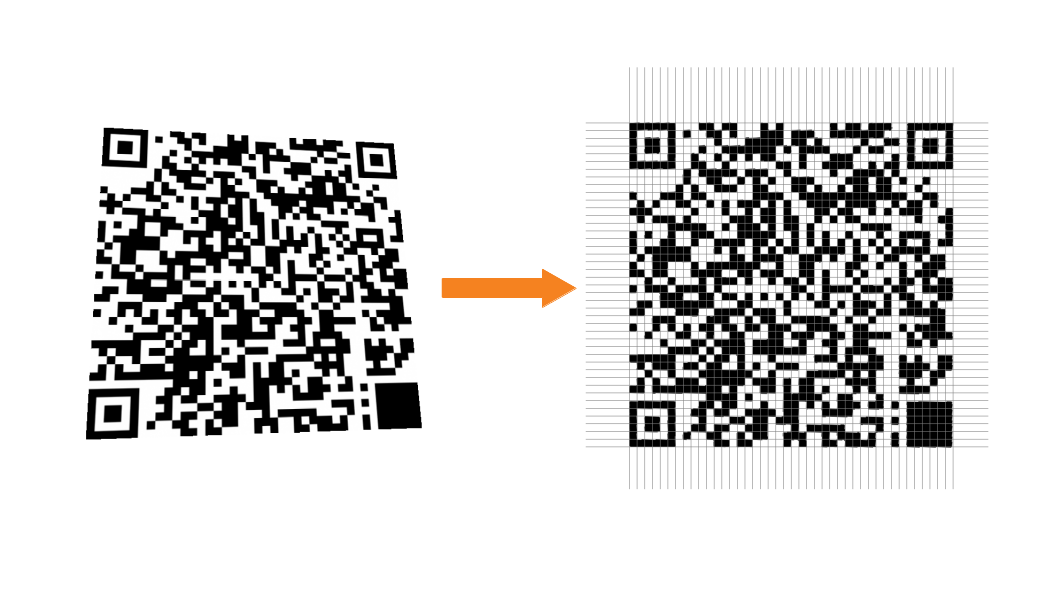
\includegraphics[width=\linewidth]{pic-01.png}
  \caption{Homography transformation}
\end{figure}


\section{Demonstration}

\section{Example}
The feasiblity of this LRC code is tested in the hadoop file system in the following steps:
\begin{itemize}
\item Compile the whole hadoop project, package it into a native distribution and deploy the hadoop system using docker container.
\item Create an empty directory in hadoop file system. Set the erasure code policy to LRC-6-4-1024k.
\item Put an 800 MB file in the directory. The file will be encoded by LRC code into 6 data chunks and 4 parity chunks.
\item Find the physical locations of file chunks. Choose several chunks and manually delete them. 
\item Fetch the file from the hadoop file system. 
\item Verify the identity of the fetched file.
\end{itemize}


First we compile the whole hadoop project and deploy the hadoop system using docker container.
Here our LRC code configuration is composed with 6 data units and 4 parity units, thus we need to deploy 10 datanodes.\\

Type "hadoop namenode -format" and "\$HADOOP\_HOME/sbin/start-all.sh" to launch hadoop file system

Type "hdfs ec -listPolicies" to check if LRC policy is registered in hadoop.
% \begin{figure}[H]
%   \centering
%   \includegraphics[width=\linewidth]{test-1.png}
%   \caption{list erasure code policies}
% \end{figure}






\end{document}
